\documentclass[12pt]{article}
\usepackage[margin=2.5cm]{geometry}
\usepackage{titling}
\usepackage{enumerate}
\usepackage{graphicx}
\usepackage{mdframed}
\usepackage{amsmath}
\usepackage{listings}
\usepackage{xcolor}
\usepackage{hyperref}
\usepackage[utf]{kotex}

\definecolor{codegreen}{rgb}{0,0.6,0}
\definecolor{codegray}{rgb}{0.5,0.5,0.5}
\definecolor{codepurple}{rgb}{0.58,0,0.82}
\definecolor{backcolour}{rgb}{0.95,0.95,0.92}

\lstdefinestyle{mystyle}{
    backgroundcolor=\color{backcolour},
    commentstyle=\color{codegreen},
    keywordstyle=\color{magenta},
    numberstyle=\tiny\color{codegray},
    stringstyle=\color{codepurple},
    basicstyle=\ttfamily\footnotesize,
    breakatwhitespace=false,
    breaklines=true,
    captionpos=b,
    keepspaces=true,
    numbers=left,
    numbersep=5pt,
    showspaces=false,
    showstringspaces=false,
    showtabs=false,
    tabsize=1
}

\lstset{style=mystyle}

\predate{}
\postdate{}

\begin{document}
\title{Lab 5: Linked Lists Solution}
\date{}
\maketitle

\section*{4) Additional exercises}
\subsection*{Generalizing \textit{\_\_getitem\_\_}}
The implementation we’ve provided for \textit{\_\_getitem\_\_} has many shortcomings
compared to Python’s built-in lists.

\bigskip

\noindent Two features that it doesn’t currently support are negative indexes and slices
(e.g., \textit{my\_list[2:5]}).

\bigskip

\noindent Your first task here is to investigate the different ways in which Python
supports these operations for built-in Python lists; you can do this by experimenting
yourself in the Python console, or by doing some reading online.

\bigskip

\noindent Then, modify the linked list implementation of \textit{\_\_getitem\_\_}
so that it handles both negative indexes and slices.

\bigskip

\noindent Note that a slice in Python is actually a class: the expression
\textit{my\_list[2:5]} is equivalent to \textit{my\_list.\_\_getitem\_\_(slice(2, 5))}.

\bigskip

\noindent Use \textit{isinstance} to determine whether the input to \textit{\_\_getitem\_\_}
is an integer or a slice.

\bigskip

\noindent The fully general method signature of \textit{\_\_getitem\_\_} should
become:

\bigskip

\begin{lstlisting}[language=python]
    def __getitem__(self, index: Union[int, slice]) -> Union[Any, LinkedList]
\end{lstlisting}

\bigskip

\noindent Note: slicing should always return a new \textit{LinkedList} object.

\bigskip

\noindent This means that for a given slice, you’ll need to create a \textit{LinkedList} and new
\textit{\_Nodes} as well, in a similar manner to how you implemented the more
powerful initializer at the end of Task 1.

\bigskip

\begin{mdframed}

\underline{\textbf{Negative Index:}}

\begin{lstlisting}[language=python,caption={task\_4\_part\_1\_solution.py}]
    class LinkedList:
    ...
        def __getitem__(self, index: int) -> Any:
            """Return the item at position <index> in this list.

            Raise IndexError if <index> is >= the length of this list.

            >>> lst = LinkedList([1, 2, 10, 200])
            >>> lst[-1]
            200
            >>> lst[2]
            10
            >>> lst[-10]
            Traceback (most recent call last):
                ...
            IndexError
            >>> str(lst[:2])
            '[1 -> 2]'
            >>> str(lst[10:1:-1])
            '[200 -> 10]'
            """
            curr = self._first
            curr_index = 0
            # ============= (Task 4, Part 1) =============
            index = index if index >= 0 else self._length + index

            if index < 0:
                raise IndexError
            # ============================================

            while curr is not None and curr_index < index:
                curr = curr.next
                curr_index += 1

            assert curr is None or curr_index == index

            if curr is None:
                raise IndexError
            else:
                return curr.item

\end{lstlisting}

\bigskip

\underline{\textbf{Slices:}}

\bigskip

\begin{lstlisting}[language=python,caption={task\_4\_part\_1\_solution.py}]
    class LinkedList:
    ...
        # ============= (Task 4, Part 1) =============
        def __getitem__(self, index: Union[int , slice]) -> Union[Any , LinkedList]:
            """Return the item at position <index> in this list.

            Raise IndexError if <index> is >= the length of this list.

            >>> lst = LinkedList([1, 2, 10, 200])
            >>> lst[-1]
            200
            >>> lst[2]
            10
            >>> lst[-10]
            Traceback (most recent call last):
                ...
            IndexError
            >>> str(lst[:2])
            '[1 -> 2]'
            >>> str(lst[10:1:-1])
            '[200 -> 10]'
            """

            if isinstance(index, slice):
                curr = self._first
                curr_index = 0
                start, stop, step = index.indices(len(self))
                # 1. initialize list
                i_list = range(start, stop, step)
                result = []

                for i in i_list:
                    # 2. fetch value from linked list
                    try:
                        item = self[i]

                        # 3. if it exists, insert to result
                        result.append(item)
                    except IndexError:
                        # 4. if it doesn't exist, then continue
                        continue

                return LinkedList(result)

            else:
                curr = self._first
                curr_index = 0
                index = index if index >= 0 else self._length + index

                if index < 0:
                    raise IndexError

                while curr is not None and curr_index < index:
                    curr = curr.next
                    curr_index += 1

                assert curr is None or curr_index == index

                if curr is None:
                    raise IndexError
                else:
                    return curr.item
        # ============================================
\end{lstlisting}
\end{mdframed}


\subsection*{Matplotlib Practice}
Use \textit{matplotlib} to plot the results of your timing experiments, using the same
approach as last week (See matplotlib section in lab 4).


\begin{mdframed}
    \begin{lstlisting}[language=python,caption={task\_4\_part\_2\_solution.py}]
    """CSC148 Lab 5: Linked Lists

    === CSC148 Winter 2020 ===
    Department of Computer Science,
    University of Toronto

    === Module description ===
    This module runs timing experiments to determine how the time taken
    to call `len` on a Python list vs. a LinkedList grows as the list size grows.
    """
    from timeit import timeit
    from task_4_part_1_solution import LinkedList
    import matplotlib.pyplot as plt

    NUM_TRIALS = 3000                        # The number of trials to run.
    SIZES = [1000, 2000, 4000, 8000, 16000]  # The list sizes to try.

    def profile_getitem(list_class: type, size: int) -> float:
        """Return the time taken to call len on a list of the given class and size.

        Precondition: list_class is either list or LinkedList.
        """
        # TODO: Create an instance of list_class containing <size> 0's.
        my_list = LinkedList([0 for x in range(size)])

        # TODO: call timeit appropriately to check the runtime of len on the list.
        # Look at the Lab 4 starter code if you don't remember how to use timeit:
        # https://www.teach.cs.toronto.edu/~csc148h/winter/labs/w4_ADTs/starter-code/timequeue.py

        time = timeit('my_list[-1]', number=1, globals=locals())

        return time

    def profile_slice(list_class: type, size: int) -> float:
        """Return the time taken to call len on a list of the given class and size.

        Precondition: list_class is either list or LinkedList.
        """
        # TODO: Create an instance of list_class containing <size> 0's.
        my_list = LinkedList([0 for x in range(size)])
        n = len(my_list)

        # TODO: call timeit appropriately to check the runtime of len on the list.
        # Look at the Lab 4 starter code if you don't remember how to use timeit:
        # https://www.teach.cs.toronto.edu/~csc148h/winter/labs/w4_ADTs/starter-code/timequeue.py

        time = timeit('my_list[n::-1]', number=1, globals=locals())

        return time



    if __name__ == '__main__':
        getitem_time_list = []
        slice_time_list = []

        for list_class in [LinkedList]:
            # Try each list size
            print('=========== __getitem__ ==========')
            for s in SIZES:
                time = profile_getitem(list_class, s)
                getitem_time_list.append(time)
                print(f'[{list_class.__name__}] Size {s:>6}: {time}')

            print('=========== slice ==========')

            for s in SIZES:
                time = profile_slice(list_class, s)
                slice_time_list.append(time)
                print(f'[{list_class.__name__}] Size {s:>6}: {time}')

        ax = plt.subplot(1,1,1)

        ax1 = plt.subplot(2, 1, 1)
        plt1, = ax1.plot(SIZES, getitem_time_list, 'ro')
        ax1.legend([plt1],["'__getitem__'"], loc="lower right")
        ax1.set_ylabel ('Time (Seconds)')
        ax1.set_title('Worst-Case Algorithm Run time vs Node Size')

        ax2 = plt.subplot(2, 1, 2)
        plt2, = ax2.plot(SIZES, slice_time_list, 'bo')
        ax2.legend([plt2],["'__getitem__.slice(...)'"], loc="lower right")
        ax2.set_xlabel('Size')
        ax2.set_ylabel('Time (Seconds)')

        plt.show()
    \end{lstlisting}

    \bigskip

    \begin{center}
    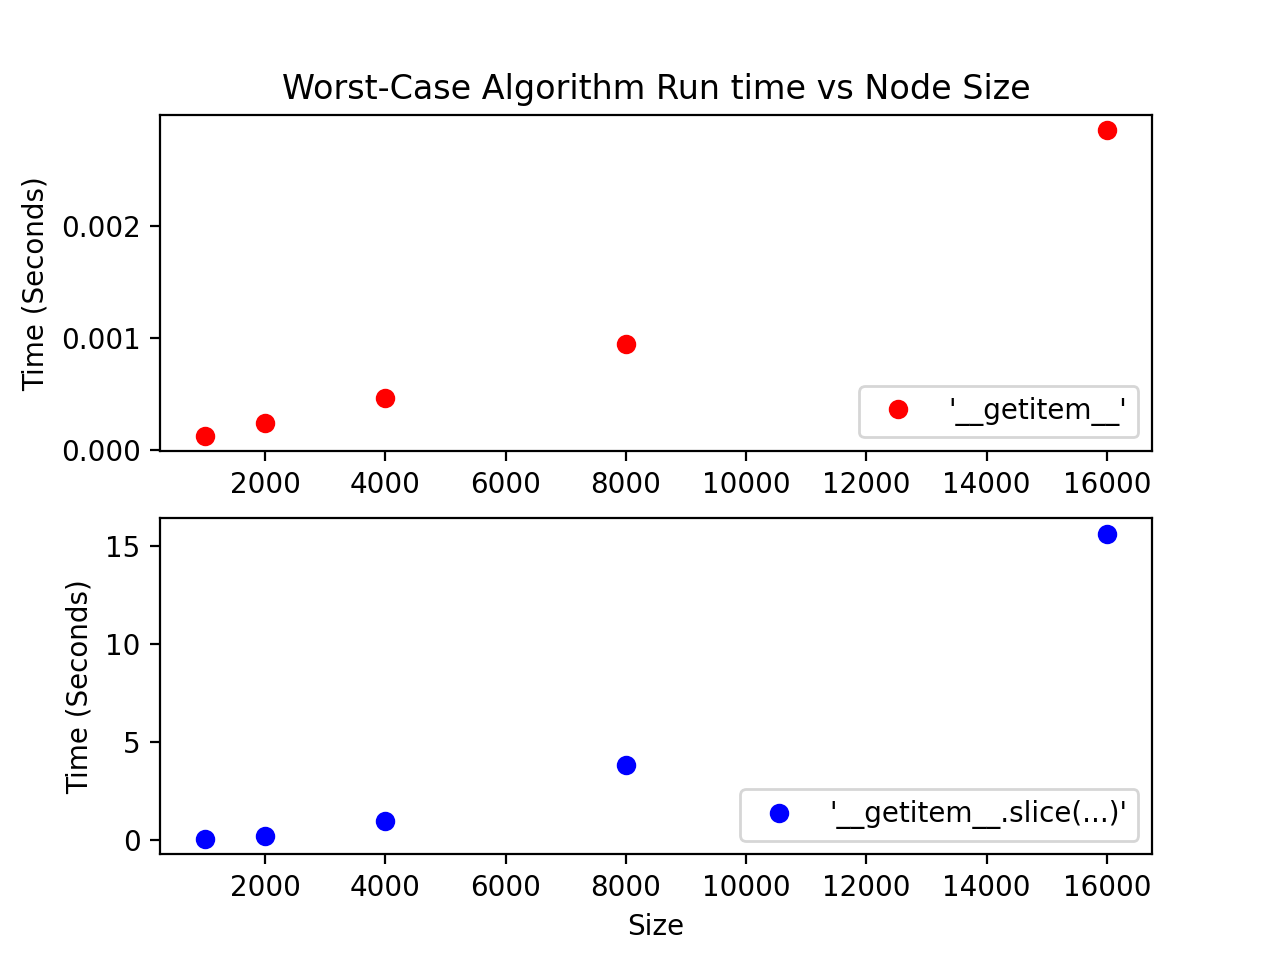
\includegraphics[width=0.8 \linewidth]{../../images/lab5_t4_s2_solution.png}
    \end{center}
\end{mdframed}

\end{document}
